%%%%%%%%%%%%%%%%%%%%%%%%%%%%%%%%%%%%%%%%%%%%%%%%%%%%%%%%%%%%%%%%%%
%%%%%%%% ICML 2014 EXAMPLE LATEX SUBMISSION FILE %%%%%%%%%%%%%%%%%
%%%%%%%%%%%%%%%%%%%%%%%%%%%%%%%%%%%%%%%%%%%%%%%%%%%%%%%%%%%%%%%%%%

% Use the following line _only_ if you're still using LaTeX 2.09.
%\documentstyle[icml2014,epsf,natbib]{article}
% If you rely on Latex2e packages, like most moden people use this:
\documentclass{article}


% use Times
\usepackage{times}
\usepackage{geometry,amsmath}

% For figures
\usepackage{graphicx} % more modern
%\usepackage{epsfig} % less modern
\usepackage{subfigure} 


% For citations
\usepackage{natbib}

% For algorithms
\usepackage{algorithm}
\usepackage{algorithmic}

% As of 2011, we use the hyperref package to produce hyperlinks in the
% resulting PDF.  If this breaks your system, please commend out the
% following usepackage line and replace \usepackage{icml2014} with
% \usepackage[nohyperref]{icml2014} above.
%\usepackage{hyperref}

% Packages hyperref and algorithmic misbehave sometimes.  We can fix
% this with the following command.
\newcommand{\theHalgorithm}{\arabic{algorithm}}

% Employ the following version of the ``usepackage'' statement for
% submitting the draft version of the paper for review.  This will set
% the note in the first column to ``Under review.  Do not distribute.''
\usepackage{icml2014}


% The \icmltitle you define below is probably too long as a header.
% Therefore, a short form for the running title is supplied here:
\icmltitlerunning{de Villalobos, Lautman, Yim}

%%%%%%%%%% Start TeXmacs macros
\newcommand{\nosymbol}{}
\newcommand{\tmop}[1]{\ensuremath{\operatorname{#1}}}
%%%%%%%%%% End TeXmacs macros

\begin{document} 

\twocolumn[
\icmltitle{Penn Project Report\\Machine Learning in Real Time Character Recognition}

% It is OKAY to include author information, even for blind
% submissions: the style file will automatically remove it for you
% unless you've provided the [accepted] option to the icml2014
% package.
\icmlauthor{Francisco de Villalobos}{frade@seas.upenn.edu}
\icmlauthor{Michael Lautman}{mlautman@seas.upenn.edu}
\icmlauthor{Justin Yim}{yimj@seas.upenn.edu}

% You may provide any keywords that you 
% find helpful for describing your paper; these are used to populate 
% the "keywords" metadata in the PDF but will not be shown in the document
\icmlkeywords{machine learning, character recognition, kaman filter}


\vskip 0.3in
]

\begin{abstract} 
This paper presents a MEMS based digital pen for handwriting recognition. While there are several devices which are capable of digitizing handwritten notes, all commercially available devices require secondary hardware to function. We propose a single device solution for digitizing text as it is written on a page. Our device tracks it's motion and uses machine learning methods to identify written characters in real time. By solving for the dynamics of the system, and using them in our Kalman Filter, we are able to estimate the pen tip accelerations and rotations as a function of time. We will use this data to compare several machine learning algorithms based on their ability to recgnize handwritten characters. 
\end{abstract} 



\section{Prototype}
In this section we give a brief summary of the hardware incorporated into the proposed device. We first describe the mechanical device before then discussing the electronics. 

\subsection{Hardware}
The pen layout and body was designed in CAD (pictured below) to ensure appropriate packing of components. The clear body was 3D printed in ABS in the University's prototyping labs. 

\begin{figure}[H]
	\centering
	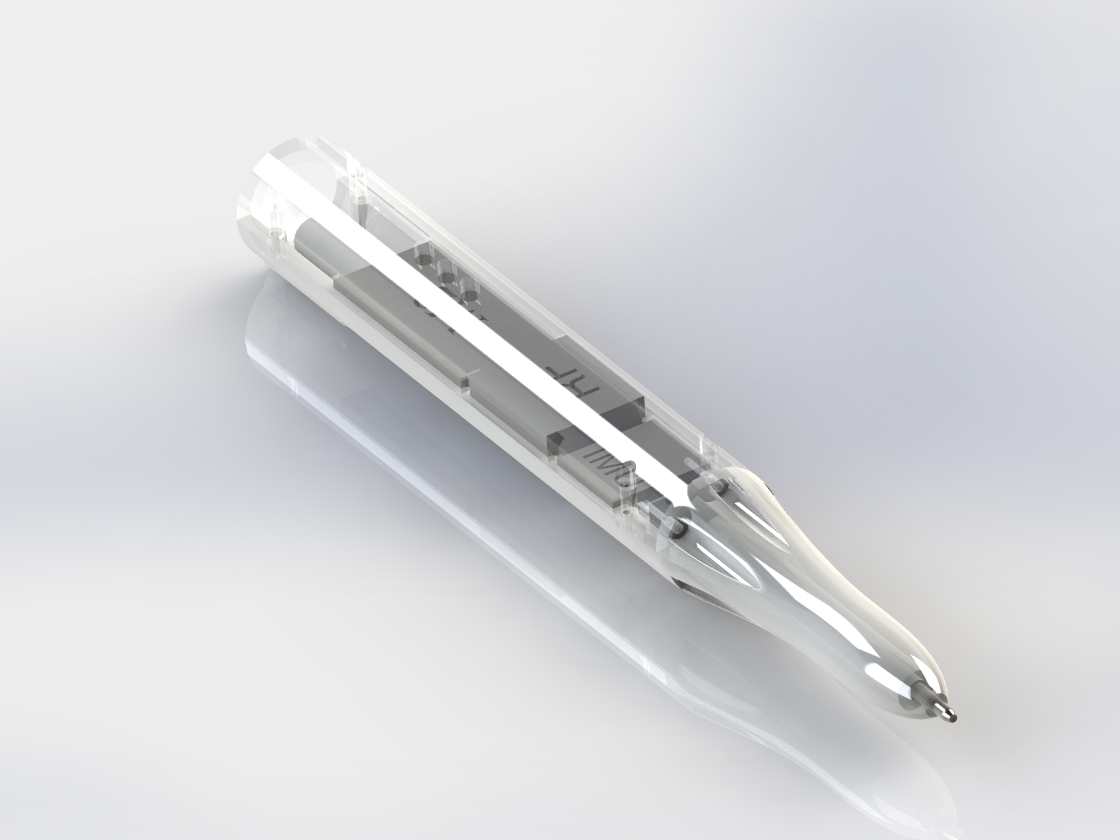
\includegraphics[width=0.5\textwidth, height= 5cm]{pen_render.png}
	\caption{Rendering of the 3D printed model of the penn}
\end{figure}

\subsection{Electronics}
An ATMega32u4 microcontroller provides on-board processing and interfaces to the wireless module, IMU, switch, and indicator LEDs. Two Nordic nRF24LE1 transceivers handle wireless communication between the pen and base station computer. Inertial measurements are provided by an MPU6050 digital IMU with configurable gain triaxial accelerometers and gyroscopes. A Honeywell HMC5883L triaxial magnetometer provides a reference to earth's magnetic field for orientation. A switch behind the pen tip detects contact with the page for character segmentation. Three LEDs on the case display pen state. The pen also includes on-board batteries, power management, and an on-off switch.

\subsection{Filtering the data}

The raw data from the IMU pose issues for learning algorithms. Sources of variance can include posture, handed-ness, roll angle of the pen, and sensor drift. To minimize sources of error, we compute the trajectory of the pen tip on the page. Using various filtering and sensor fusion techniques we are able to compensate for gravity and perform attitude and position estimation. We use a Kalman Filter to estimate the orientation of the pen relative to gravity so that we can subtract the gravity components from the acceleration measurements. 

\subsection{Coordinate Transformation}
Accelerations and rotations of the pen body measured at the IMU are translated to the tip by the following transform:

\textbf{P}: location of the IMU \\
\textbf{O}: origin of frame G on the page \\
\textbf{frame G}: SRT fixed to the page with origin O (ground frame) \\
\textbf{frame M}: SRT fixed to the pen at the IMU with origin at point P (pen frame) \\
\textbf{Q}: location of the pen tip \\
$\underset{\mbox{\textasciitilde}}{\tmop{\textbf{PQ}}}$: vector from the IMU origin to
the pen tip

The acceleration of the pen tip in the ground frame is given by:
\begin{align*}
  ^G \underset{\mbox{\textasciitilde}}{a}^Q =^G
  \underset{\mbox{\textasciitilde}}{a}^P +^M
  \underset{\mbox{\textasciitilde}}{a}^Q &+^G
  \underset{\mbox{\textasciitilde}}{\alpha}^P \times
  \underset{\mbox{\textasciitilde}}{\tmop{PQ}} + 2^G
  \underset{\mbox{\textasciitilde}}{w}^M \times^M
  \underset{\mbox{\textasciitilde}}{v}^Q + ... \\ &+ ^G 
  \underset{\mbox{\textasciitilde}}{w}^M \times \left(^G
  \underset{\mbox{\textasciitilde}}{w}^M \times
  \underset{\mbox{\textasciitilde}}{\tmop{PQ}} \right)
\end{align*}
Since point Q (the pen tip) is fixed in frame M (the pen frame), $^M
\underset{\mbox{\textasciitilde}}{a}^Q$ and $^M
\underset{\mbox{\textasciitilde}}{v}^Q$ are both 0. The above equation simplifies to:
\begin{eqnarray*}
  & ^G \underset{\mbox{\textasciitilde}}{a}^Q =^G
  \underset{\mbox{\textasciitilde}}{a}^P +^G
  \underset{\mbox{\textasciitilde}}{\alpha}^P \times
  \underset{\mbox{\textasciitilde}}{\tmop{PQ}} +^G
  \underset{\mbox{\textasciitilde}}{w}^M \times \left(^G
  \underset{\mbox{\textasciitilde}}{w}^M \times
  \underset{\mbox{\textasciitilde}}{\tmop{PQ}} \right) & 
\end{eqnarray*}
The IMU measures accelerations and angular velocities of frame M relative to frame G expressed in frame M. \ Using the attitude estimate, these measurements can be rotated into frame G to produce $^G
\underset{\mbox{\textasciitilde}}{a}^P$ and $^G
\underset{\mbox{\textasciitilde}}{w}^M \nosymbol$. \ The angular acceleration
$^G \underset{\mbox{\textasciitilde}}{\alpha}^P$ is obtained by numerically
differentiating $^G \underset{\mbox{\textasciitilde}}{w}^M$.

The trajectory of the pen tip in the page frame is obtained by twice-integrating $^G \underset{\mbox{\textasciitilde}}{a}^Q$.
Since the velocity and position are integrations of noisy signals they are prone to very significant drift over time. To counteract this drift, the position and velocity estimates are re-zeroed at the start of every character and both the velocity and position are high pass filtered. The resulting trajectory can be plotted in the plane to approximate the appearance of the character on the page. This trajectory image is sampled to produce a black and white image which is then scaled and blurred to produce the final learning features.
 
\subsection{Preliminary Results}
We are currently able to produce relatively accurate trajectory estimates. The integrated character image is prone to distortion due to velocity and position drift over the course of writing the character. Our current filtering schemes are somewhat successful at reducing integration drift and rejecting noise from vibration. Figure 2 shows a trajectory recovered 'g' that we were able to produce using our methodology.

\begin{figure}[H]
\centering
    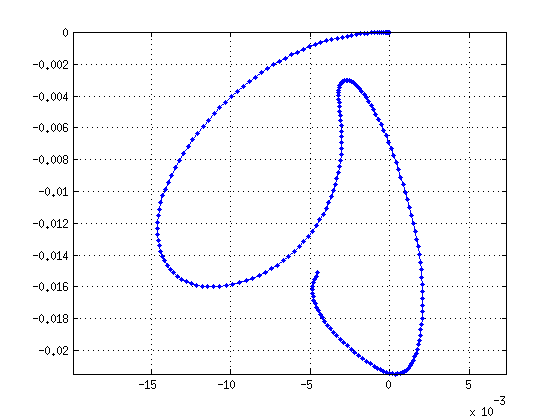
\includegraphics[width=0.5\textwidth, height= 5cm]{g.png}
    \caption{Recovered letter "g"}
\end{figure}


\subsection{Next Steps}
The next step in the project is to create a labeled test set. With a training set in hand, we will begin testing different learning algorithms so that we can find the most successful model. To this end, we will approach the learning component of this project in two ways. One method involves projecting the trajectory into an image and using learning algorithms such as neural networks. The other method involves using feature selection methods on the filtered signals before integration and differentiation. This method will require that we transform the time series data into a constant width feature vector. By interpolating, we are able to produce this result. Reducing dimensionality might prove to be an important step if we experience performance issues. In that case we intend to use either PCA or LDA to generate features. We intend to test the performance of various learning algorithms including Hidden Markov Models, Neural Networks, and Naive Bayes.
 
\section*{Acknowledgments} 
 
Attitude estimation Kalman Filter and initial approximation provided by \textbf{open-source} code from Sebastian Madgwick (July 2012), based on his paper \textbf{Estimation of IMU and MARG orientation using a gradient descent algorithm}.\\\\
For trajectory reconstruction, consulted Jeen-Shing Wang, Yu-Liang Hsu, and Jiun-Nan Liu's paper entitled \textbf{An Inertial-Measurement-Unit-Based Pen With a Trajectory Reconstruction Algorithm and Its Applications}.
%\bibliography{example_paper}
%\bibliographystyle{icml2014}

\end{document} 


% This document was modified from the file originally made available by
% Pat Langley and Andrea Danyluk for ICML-2K. This version was
% created by Lise Getoor and Tobias Scheffer, it was slightly modified  
% from the 2010 version by Thorsten Joachims & Johannes Fuernkranz, 
% slightly modified from the 2009 version by Kiri Wagstaff and 
% Sam Roweis's 2008 version, which is slightly modified from 
% Prasad Tadepalli's 2007 version which is a lightly 
% changed version of the previous year's version by Andrew Moore, 
% which was in turn edited from those of Kristian Kersting and 
% Codrina Lauth. Alex Smola contributed to the algorithmic style files.  
